% !TEX TS-program = pdflatex
% !TEX encoding = UTF-8 Unicode

\documentclass[a4paper, titlepage=false, parskip=full-, 10pt]{scrartcl}

\usepackage[utf8]{inputenc}
\usepackage[T1]{fontenc}
\usepackage[english, ngerman]{babel}
\usepackage{babelbib}
\usepackage{hyperref}
\usepackage{listings}
\usepackage{framed}
\usepackage{color}
\usepackage{graphicx}
\usepackage[normalem]{ulem}
\usepackage{cancel}
\usepackage{array}
\usepackage{amsmath}
\usepackage{amssymb}
\usepackage{amsthm}
\usepackage{algorithm}
\usepackage{algorithmic}
\usepackage{geometry}
\usepackage{subfigure}
\geometry{a4paper, top=20mm, left=35mm, right=25mm, bottom=40mm}

\newcounter{tasknbr}
\setcounter{tasknbr}{1}
\newenvironment{task}[1]{{\bf Aufgabe \arabic {tasknbr}\stepcounter{tasknbr}} (#1):\begin{enumerate}}{\end{enumerate}}
\newcommand{\subtask}[1]{\item[#1)]}

% Listings -----------------------------------------------------------------------------
\definecolor{red}{rgb}{.8,.1,.2}
\definecolor{blue}{rgb}{.2,.3,.7}
\definecolor{lightyellow}{rgb}{1.,1.,.97}
\definecolor{gray}{rgb}{.7,.7,.7}
\definecolor{darkgreen}{rgb}{0,.5,.1}
\definecolor{darkyellow}{rgb}{1.,.7,.3}
\lstloadlanguages{C++,[Objective]C,Java}
\lstset{
escapeinside={§§}{§§},
basicstyle=\ttfamily\footnotesize\mdseries,
columns=fullflexible,
keywordstyle=\bfseries\color{blue},
commentstyle=\color{darkgreen},      
stringstyle=\color{red},
numbers=left,
numberstyle=\ttfamily\scriptsize\color{gray},
breaklines=true,
showstringspaces=false,
tabsize=4,
captionpos=b,
float=htb,
frame=tb,
frameshape={RYR}{y}{y}{RYR},
rulecolor=\color{black},
xleftmargin=15pt,
xrightmargin=4pt,
aboveskip=\bigskipamount,
belowskip=\bigskipamount,
backgroundcolor=\color{lightyellow},
extendedchars=true,
belowcaptionskip=15pt}

%% Enter current values here: %%
\newcommand{\lecture}{Robotik WS15/16}
\newcommand{\tutor}{}
\newcommand{\assignmentnbr}{11}
\newcommand{\students}{Julius Auer, Thomas Tegethoff}
%%-------------------------------------%%

\begin{document}  
{\small \textsl{\lecture \hfill \tutor}}
\hrule
\begin{center}
\textbf{Übungsblatt \assignmentnbr}\\
[\bigskipamount]
{\small \students}
\end{center}
\hrule

\begin{task}{RRT 1}
\item[]
Wir samplen gleichverteilt (auch die Zielposition wird nicht bevorzugt).

Liegt ein Sample weiter vom nächsten Nachbarn entfernt als die maximale Schrittweite $s=5$, wird der neue Knoten ''herangezogen''.

Wir gehen über maximal $n=1000$ Iterationen (nicht so viele, damit man ein paar ''gute'' Kanten sehen kann).

Der Algo verhält sich genau wie erwartet. Besonders ''schön'' ist (b), wo ein offensichtlich nicht optimaler Weg gefunden wurde. Ergebnisse zeigt Abbildung \ref{fig:1}.

\begin{figure}[!htpb]
\centering
\subfigure[$t=(30,15)$]{
  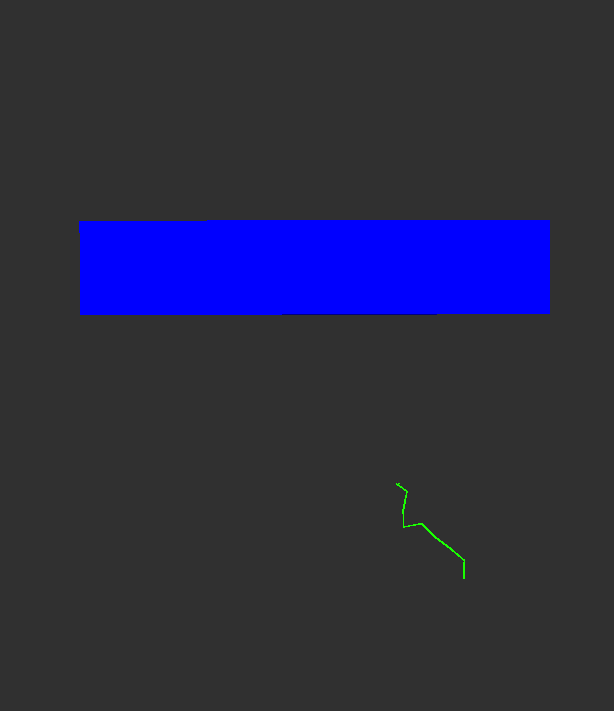
\includegraphics[width=0.48\linewidth]{capture_1-1}
}
\subfigure[$t=(0,25)$]{
  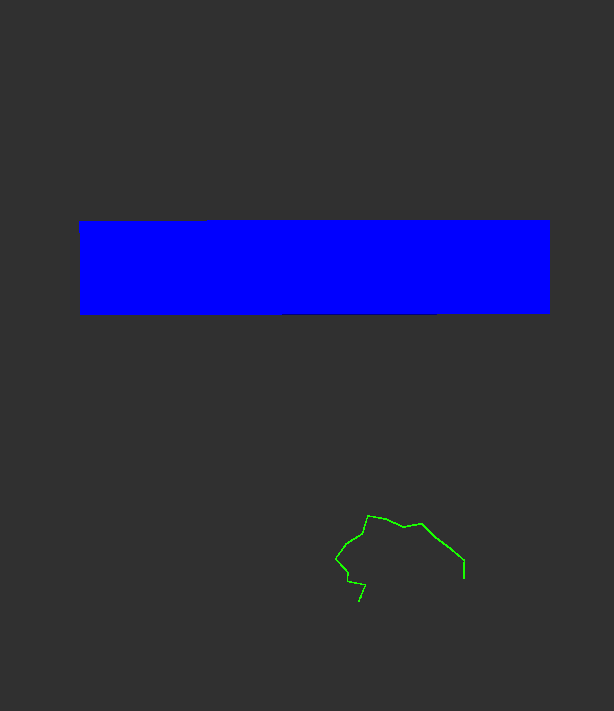
\includegraphics[width=0.48\linewidth]{capture_1-2}
}
\subfigure[$t=(35,50)$]{
  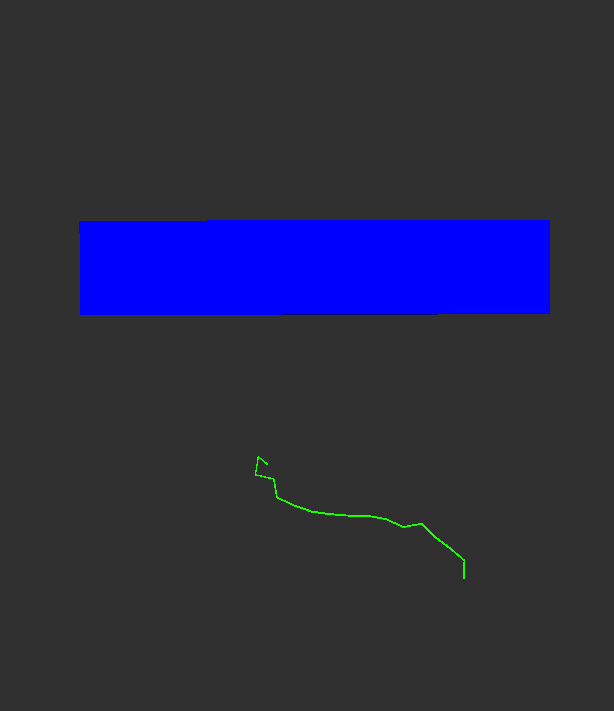
\includegraphics[width=0.48\linewidth]{capture_1-3}
}
\subfigure[$t=(150,75)$]{
  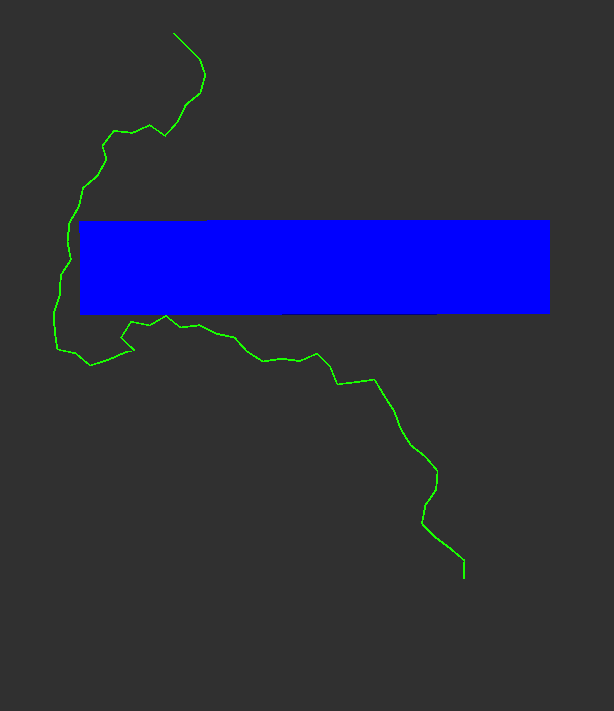
\includegraphics[width=0.48\linewidth]{capture_1-4}
}
\caption{Pfade aus RRT}
\label{fig:1}
\end{figure}
\end{task}

\begin{task}{RRT 2}
\item[]
Wir nutzen zwar den alten PID, aufgrund der niedrigen Geschwindigkeiten ist dessen Auswirkung aber marginal - ein $(1,0,0)$-PID funktioniert hier genauso gut wie jeder andere auch. Wir fahren halt sehr langsam.

Wir fahren - wie vorgeschlagen - stets den nächstem Punkt auf dem geplanten Pfad an, bis wir ''nah genug'' sind ($d=2$).

Abbildung \ref{fig:2} zeigt die aktuelle Position des Autos $(cur_x,cur_y)$ die sich stets dem nächsten Punkt auf dem geplanten Pfad $(tar_x,tar_y)$ nähert. Da der Plot sehr breit ist, ist nur ein Ausschnitt abgebildet.

\begin{figure}[!htpb]
\centering
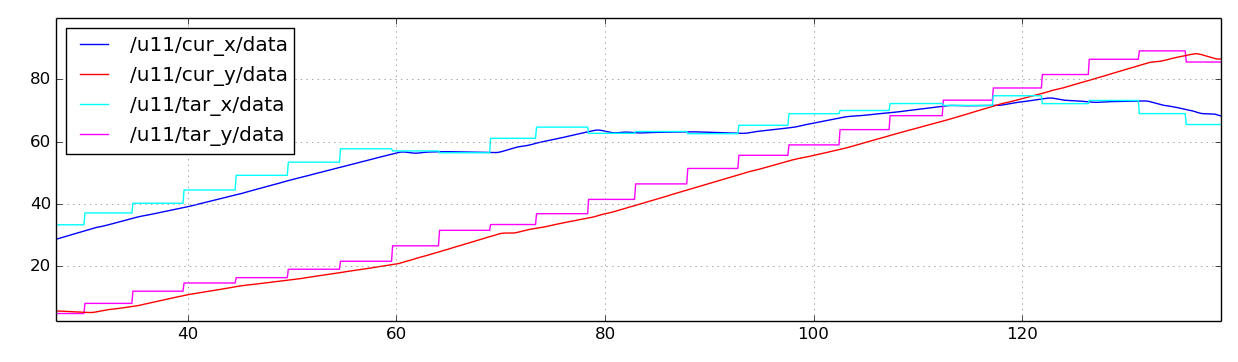
\includegraphics[width=1.1\linewidth]{capture_2-1}
\caption{Geplanter Pfad und tatsächliche Position über Zeit}
\label{fig:2}
\end{figure}
\end{task}
\end{document}